\ChapterImageStar[cap:validacion]{Implementación y validación de la solución}{./images/fondo.png}\label{cap:validacion}
\mbox{}\\
En este capítulo se detalla el proceso de validación de la solución propuesta, que incluye tanto pruebas técnicas como la aceptación por parte del cliente. 
\section{Pruebas de validacion técnica}\label{sec:functional-tests}

%=========================functional-test/backup=========================
\subsection{functional-test/backup}\label{sec:functional-test-backup}
\noindent
La siguiente sección presenta los distintos manifiestos y scripts que conforman la estrategia de creación de respaldo en Kubernetes. Cada archivo cumple un rol específico dentro del despliegue, desde la definición del pod y sus volúmenes. A continuación, se describen brevemente los archivos incluidos en este paquete:
\subsubsection{deployment.yaml}
\noindent
El siguiente manifiesto en formato \texttt{YAML} define un recurso de tipo \texttt{Deployment} en Kubernetes para la aplicación \texttt{nginx}. Este despliegue solicita que exista al menos una réplica en ejecución, gestionada automáticamente por el controlador de Kubernetes. Además, se especifican etiquetas para la selección de pods, la imagen utilizada del contenedor, los puertos expuestos y un volumen persistente que se monta en el directorio \texttt{/usr/share/nginx/html}, el cual permite servir archivos estáticos de manera persistente.

\begin{minted}[frame=lines,
    fontsize=\scriptsize,
    breaklines]{yaml}
apiVersion: apps/v1             # Versión de la API de Kubernetes utilizada para el recurso
kind: Deployment                # Tipo de recurso: Deployment (gestiona pods y réplicas)
metadata:
  name: nginx-deployment        # Nombre asignado al Deployment
spec:
  replicas: 1                   # Número de réplicas del pod
  selector:
    matchLabels:
      app: nginx                # Selector para identificar los pods asociados
  template:                     # Plantilla que define cómo serán los pods
    metadata:
      labels:
        app: nginx              # Etiquetas aplicadas al pod
    spec:
      containers:
        - name: nginx           # Nombre del contenedor
          image: nginx:stable   # Imagen de Docker utilizada
          ports:
            - containerPort: 80 # Puerto expuesto por el contenedor (HTTP)
          volumeMounts:
            - name: nginx-storage
              mountPath: /usr/share/nginx/html  # Montaje del volumen para archivos estáticos
      volumes:
        - name: nginx-storage
          persistentVolumeClaim:
            claimName: nginx-pvc # Reclamo de volumen persistente asociado
\end{minted}

\subsubsection{pv.yaml}
\noindent
El siguiente manifiesto en \texttt{YAML} define un recurso de tipo \texttt{PersistentVolume} (PV) en Kubernetes, 
el cual representa una pieza de almacenamiento en el clúster que puede ser reclamada por los pods mediante 
un \texttt{PersistentVolumeClaim} (PVC). En este caso, el volumen tiene una capacidad de \texttt{1Gi}, con 
modo de acceso \texttt{ReadWriteOnce}, lo que significa que puede ser montado en modo lectura y escritura por 
un único nodo al mismo tiempo. La configuración utiliza un \texttt{hostPath}, lo que enlaza el volumen a una 
ruta del sistema de archivos del nodo anfitrión (\texttt{/mnt/data/nginx}).

\begin{minted}[frame=lines,
    fontsize=\scriptsize,
    breaklines]{yaml}
apiVersion: v1                # Versión de la API de Kubernetes para recursos básicos
kind: PersistentVolume         # Tipo de recurso: PersistentVolume (PV)
metadata:
  name: nginx-pv               # Nombre asignado al volumen persistente
spec:
  capacity:
    storage: 1Gi               # Capacidad de almacenamiento asignada al volumen
  accessModes:
    - ReadWriteOnce            # Permite acceso de lectura/escritura desde un solo nodo
  hostPath:                    # Define un path físico en el nodo (útil en pruebas locales)
    path: /mnt/data/nginx      # Ruta en el sistema de archivos del nodo donde se almacena el volumen
\end{minted}
\subsubsection{service.yaml}
\noindent
Este archivo YAML define un recurso \texttt{PersistentVolumeClaim (PVC)}, que permite a los pods solicitar almacenamiento persistente de acuerdo con lo especificado en un \texttt{PersistentVolume (PV)} previamente configurado. En este caso, el PVC solicita \texttt{1~GiB} de almacenamiento con modo de acceso \texttt{ReadWriteOnce}, lo que significa que solo un nodo podrá montar el volumen en modo lectura y escritura de manera simultánea. El PVC funciona como una capa intermedia entre los pods y el PV, desacoplando la aplicación de los detalles específicos de la infraestructura de almacenamiento.

\begin{minted}[frame=lines,
    fontsize=\scriptsize,
    breaklines]{yaml}
apiVersion: v1
kind: PersistentVolumeClaim
metadata:
  name: nginx-pvc
spec:
  accessModes:
    - ReadWriteOnce
  resources:
    requests:
      storage: 1Gi
\end{minted}
\subsubsection{writer-pod.yaml}
\noindent
Este manifiesto define un \texttt{Pod} denominado \texttt{writer-pod}, cuyo propósito es servir como contenedor de prueba para validar la persistencia de datos en Kubernetes. El pod utiliza la imagen ligera \texttt{busybox}, ejecutándose en segundo plano mediante el comando \texttt{sleep} para mantenerse activo. Además, monta un volumen persistente a través del \texttt{PersistentVolumeClaim} \texttt{nginx-pvc}, asignando la ruta interna \texttt{/data}. De esta manera, cualquier dato escrito en dicho directorio dentro del pod se almacenará en el volumen persistente, permitiendo comprobar la correcta configuración de la capa de almacenamiento.

\begin{minted}[frame=lines,
    fontsize=\scriptsize,
    breaklines]{yaml}
apiVersion: v1
kind: Pod
metadata:
  name: writer-pod
spec:
  containers:
    - name: writer
      image: busybox
      command: [ "sleep", "3600" ]  # mantiene el pod activo
      volumeMounts:
        - mountPath: /data          # directorio donde se montará el PVC
          name: nginx-storage
  volumes:
    - name: nginx-storage
      persistentVolumeClaim:
        claimName: nginx-pvc        # vínculo al PVC previamente creado
\end{minted}

\subsubsection{run-tests.sh}
\noindent
Este script en bash automatiza el proceso de validación funcional de un entorno de Kubernetes desplegado en un clúster virtual. Primero realiza el arranque de las máquinas virtuales del clúster y carga los archivos \texttt{.yaml} necesarios para el despliegue de recursos (deployment, volúmenes persistentes, servicio y un pod de prueba denominado \texttt{writer-pod}). Luego, espera hasta que dicho pod se encuentre en estado \texttt{Running}, tras lo cual se ejecutan comandos dentro de él para crear archivos de prueba en el volumen asociado. Finalmente, el script realiza respaldos tanto a nivel del volumen persistente \texttt{(PVC)} como directamente desde el pod, verificando la integración de la capa de almacenamiento con las aplicaciones en ejecución.

\begin{minted}[frame=lines,
    fontsize=\scriptsize,
    breaklines]{bash}
#!/bin/bash

# Muestra mensaje de inicio de arranque de VMs del clúster
echo "======= Booting vms ======="
cluster-bootup -m 1 -w 2   # Inicia 1 master y 2 workers

# Sube los manifiestos .yaml al nodo master
echo "====== Uploadindg .yaml files ========"
upload_yaml master1 deployment.yaml
upload_yaml master1 pvc.yaml
upload_yaml master1 pv.yaml
upload_yaml master1 service.yaml
upload_yaml master1 writer-pod.yaml

# Verifica el estado del pod hasta que esté en Running
echo "======= modyfing files ========"
while ! ssh-vm -r master1 -c "kubectl get pod/writer-pod" | grep -q Running 
do
   sleep 1
done

# Escribe un archivo de prueba en el volumen persistente
ssh-vm -r master1 -c "kubectl exec writer-pod -- sh -c 'echo functional test for backup > /data/dummy_file.txt'"

# Realiza respaldo del PVC asociado
echo "====== backing up for pvc ======="
backup nginx-pvc

# Escribe un archivo de prueba directamente en el pod
echo "====== backing up for pod ======="
ssh-vm -r master1 -c "kubectl exec writer-pod -- sh -c 'echo functional test for backup in a pod > /data/dummy_file_pod.txt'"

# Realiza respaldo a nivel de pod, copiando datos desde /data
backup -p writer-pod:/data
\end{minted}



%=========================functional-test/cluster-bootup=========================

\subsection{functional-test/cluster-bootup}
\noindent

\subsubsection{run-tests.sh}
\noindent
Este script en \texttt{bash} implementa un conjunto de pruebas funcionales automatizadas para verificar la correcta creación de clústeres virtuales mediante el uso de la herramienta \texttt{cluster-bootup}. Se evalúan tres configuraciones distintas: un clúster con un maestro y un trabajador, un clúster con dos maestros y un trabajador, y finalmente una variante que además incluye un servidor \texttt{NAT-Backup}. El script compara los resultados esperados con los obtenidos tras el despliegue de las máquinas virtuales, contabilizando las pruebas superadas y limpiando el clúster al finalizar cada verificación. De esta forma, se garantiza la reproducibilidad y consistencia en los entornos de prueba.  

\begin{minted}[frame=lines,
    fontsize=\scriptsize,
    breaklines]{bash}
#!/bin/bash

# Contador de pruebas exitosas
SUCCEDEED_TESTS=0

# Función de verificación: compara valores esperados con resultados
check(){
     echo +++++++++++++++++strings+++++++++++++++++++++++++
     echo $2
     echo $3
     if [[ "$2" == "$3" ]]
     then
        echo "Test for $1 succedeed"
        SUCCEDEED_TESTS=$(( $SUCCEDEED_TESTS + 1 ))
        return 0
     fi

     echo "Test for $1 failed"
     return 1
}

# ===== Primera prueba: 1 master, 1 worker =====
export EXPECTED_RESULT=" master1 NAT-Master worker1"
cluster-bootup -m 1 -w 1
export RESULT=$( get-vm | sort | tr -d '\n')
check  "1 master 1 worker" "$EXPECTED_RESULT" "$RESULT"
clean-cluster -y

# ===== Segunda prueba: 2 masters, 1 worker =====
export EXPECTED_RESULT=" load-balancer1 master1 master2 NAT-Master worker1"
cluster-bootup -m 2 -w 1
export RESULT=$( get-vm | sort | tr -d '\n')
check  "2 master 1 worker" "$EXPECTED_RESULT" "$RESULT"
clean-cluster -y

# ===== Tercera prueba: 2 masters, 1 worker, 1 NAT Backup =====
export EXPECTED_RESULT=" load-balancer1 master1 master2 NAT-Backup NAT-Master worker1"
cluster-bootup -m 2 -w 1 -b
export RESULT=$( get-vm | sort | tr -d '\n')
check  "2 master 1 worker 1 NAT Backup" "$EXPECTED_RESULT" "$RESULT"
clean-cluster -y

# Reporte final de pruebas
echo "${SUCCEDEED_TESTS}/3 tests succeeded"
\end{minted}


%=========================functional-test/get-ip=========================

\subsection{functional-test/get-ip}
\noindent

\subsubsection{run-tests.sh}
\noindent
Este script en \texttt{bash} realiza una serie de pruebas para validar la correcta creación de un clúster con dos nodos maestros, un nodo trabajador, un balanceador de carga y un servidor \texttt{NAT-Backup}. Tras ejecutar el despliegue mediante la función \texttt{cluster-bootup}, el script verifica que cada máquina virtual reciba la dirección IP correspondiente a su rol: los maestros, el trabajador y el balanceador de carga dentro de la red \texttt{192.x.x.x}, mientras que los servidores NAT deben ubicarse en la subred \texttt{172.x.x.x}. Cada prueba exitosa incrementa un contador, y al final se presenta un resumen del total de pruebas superadas.  

\begin{minted}[frame=lines,
    fontsize=\scriptsize,
    breaklines]{bash}
#!/bin/bash

# Inicia el clúster con:
# - 1 worker
# - 2 masters
# - servidor NAT de respaldo (-b)
cluster-bootup -w 1 -m 2 -b

# Breve pausa para dar tiempo a que arranquen las VMs
sleep 2

# Contador de pruebas exitosas
SUCCESS_TEST_COUNT=0

# Verificación de IPs según el rol de cada VM
get-ip master1 | grep 192 && echo "Test for master succedeed" \
  && SUCCESS_TEST_COUNT=$(( $SUCCESS_TEST_COUNT + 1 ))

get-ip worker1 | grep 192 && echo "Test for worker succedeed" \
  && SUCCESS_TEST_COUNT=$(( $SUCCESS_TEST_COUNT + 1 ))

get-ip load-balancer | grep 192 && echo "Test for load-balancer succedeed" \
  && SUCCESS_TEST_COUNT=$(( $SUCCESS_TEST_COUNT + 1 ))

get-ip NAT-Master | grep 172 && echo "Test for NAT-Master succedeed" \
  && SUCCESS_TEST_COUNT=$(( $SUCCESS_TEST_COUNT + 1 ))

get-ip NAT-Backup | grep 172 && echo "Test for NAT-Backup succedeed" \
  && SUCCESS_TEST_COUNT=$(( $SUCCESS_TEST_COUNT + 1 ))

# Resultado final de las pruebas
echo "$SUCCESS_TEST_COUNT/5 tests succedeed"
\end{minted}



%=========================functional-test/aplicar-yml=========================/

\subsection{functional-test/upload-yaml}\label{sec:functional-test-upload-yaml}

\subsubsection{test-deployment.yaml}
\noindent
Este archivo en formato \texttt{YAML} define un objeto de tipo \texttt{Deployment} en Kubernetes para desplegar una instancia de Nginx. El despliegue crea un único pod (\texttt{replicas: 1}) que utiliza la imagen estable de Nginx y expone el puerto 80 para atender solicitudes HTTP. Además, mediante la sección \texttt{selector} y las etiquetas (\texttt{labels}), se asegura la asociación entre el \texttt{Deployment} y los pods que administra, garantizando que Kubernetes mantenga en ejecución la cantidad definida de réplicas.

\begin{minted}[frame=lines,
    fontsize=\scriptsize,
    breaklines]{yaml}

apiVersion: apps/v1
kind: Deployment
metadata:
  name: nginx-deployment
spec:
  replicas: 1
  selector:
    matchLabels:
      app: nginx
  template:
    metadata:
      labels:
        app: nginx
    spec:
      containers:
        - name: nginx
          image: nginx:stable
          ports:
            - containerPort: 80

\end{minted}


\subsubsection{run-tests.sh}
\noindent
Este script en \texttt{bash} realiza una prueba funcional básica sobre un clúster recién creado. Primero levanta la infraestructura mínima con un nodo maestro y un nodo trabajador. Luego, transfiere y aplica en el maestro un archivo \texttt{YAML} que define un despliegue de prueba (\texttt{test-deployment.yaml}). Finalmente, el script comprueba si el despliegue denominado \texttt{nginx-deployment} se encuentra en ejecución mediante el comando \texttt{kubectl get pods}. Si se detecta correctamente, se imprime un mensaje de éxito; en caso contrario, se muestra un mensaje de fallo.  

\begin{minted}[frame=lines,
    fontsize=\scriptsize,
    breaklines]{bash}

#!/bin/bash

# Levanta un clúster con:
# - 1 nodo master
# - 1 nodo worker
cluster-bootup -m 1 -w 1

# Sube y aplica el archivo YAML al nodo master1
upload_yaml master1 test-deployment.yaml

# Verifica que el pod asociado al despliegue "nginx-deployment" esté corriendo.
# Si aparece en la lista de pods, la prueba es exitosa, de lo contrario falla.
ssh-vm -r master1 -c "kubectl get pods" | grep -q nginx-deployment \
    && echo "Test succedeed" \
    || echo "Test failed"

\end{minted}


\section{Demostración de la validación técnica}
\noindent
Se han documentado y registrado las pruebas técnicas realizadas para validar la solución propuesta. Esta documentación son elementos audiovisuales que evidencian la correcta implementación y funcionamiento de los componentes desarrollados. Esta Demostración puede encontrarse en el siguiente enlace: \href{https://drive.google.com/drive/folders/1UgpmFmz7E2uYxv_FCGCpYArZDIMc0nxv?usp=sharing}{aquí}


\section{Aceptación de la solución por parte del cliente}\label{sec:aceptacion-solucion}
\noindent
El día 10 de octubre se realizó la reunión formal de aceptación de la solución arquitectónica con el docente Luis Eduardo Sepúlveda Rodríguez, representante del \GRID\ para esta solución y principal \textit{stakeholder}. Durante esta sesión, se presentaron de manera integral los resultados de la investigación, los cuales demostraron cómo la solución propuesta, basada en la tecnología Containerd y el orquestador K3S. El docente representante, en su calidad de cliente, validó que el \PMV\ implementado satisface los requerimientos académicos y de investigación identificados, resaltando su reproducibilidad, el bajo consumo de recursos y su compatibilidad con la infraestructura existente de Xcp-ng. En consecuencia, se procedió a la aceptación oficial de la solución, certificando que cumple con los objetivos planteados, marcando así un hito significativo en la culminación exitosa del proyecto de tesis. En la figura~\ref{fig:aceptacion-solucion} se muestra una captura de pantalla de la reunión de aceptación.
\begin{figure}[H]
    \centering
    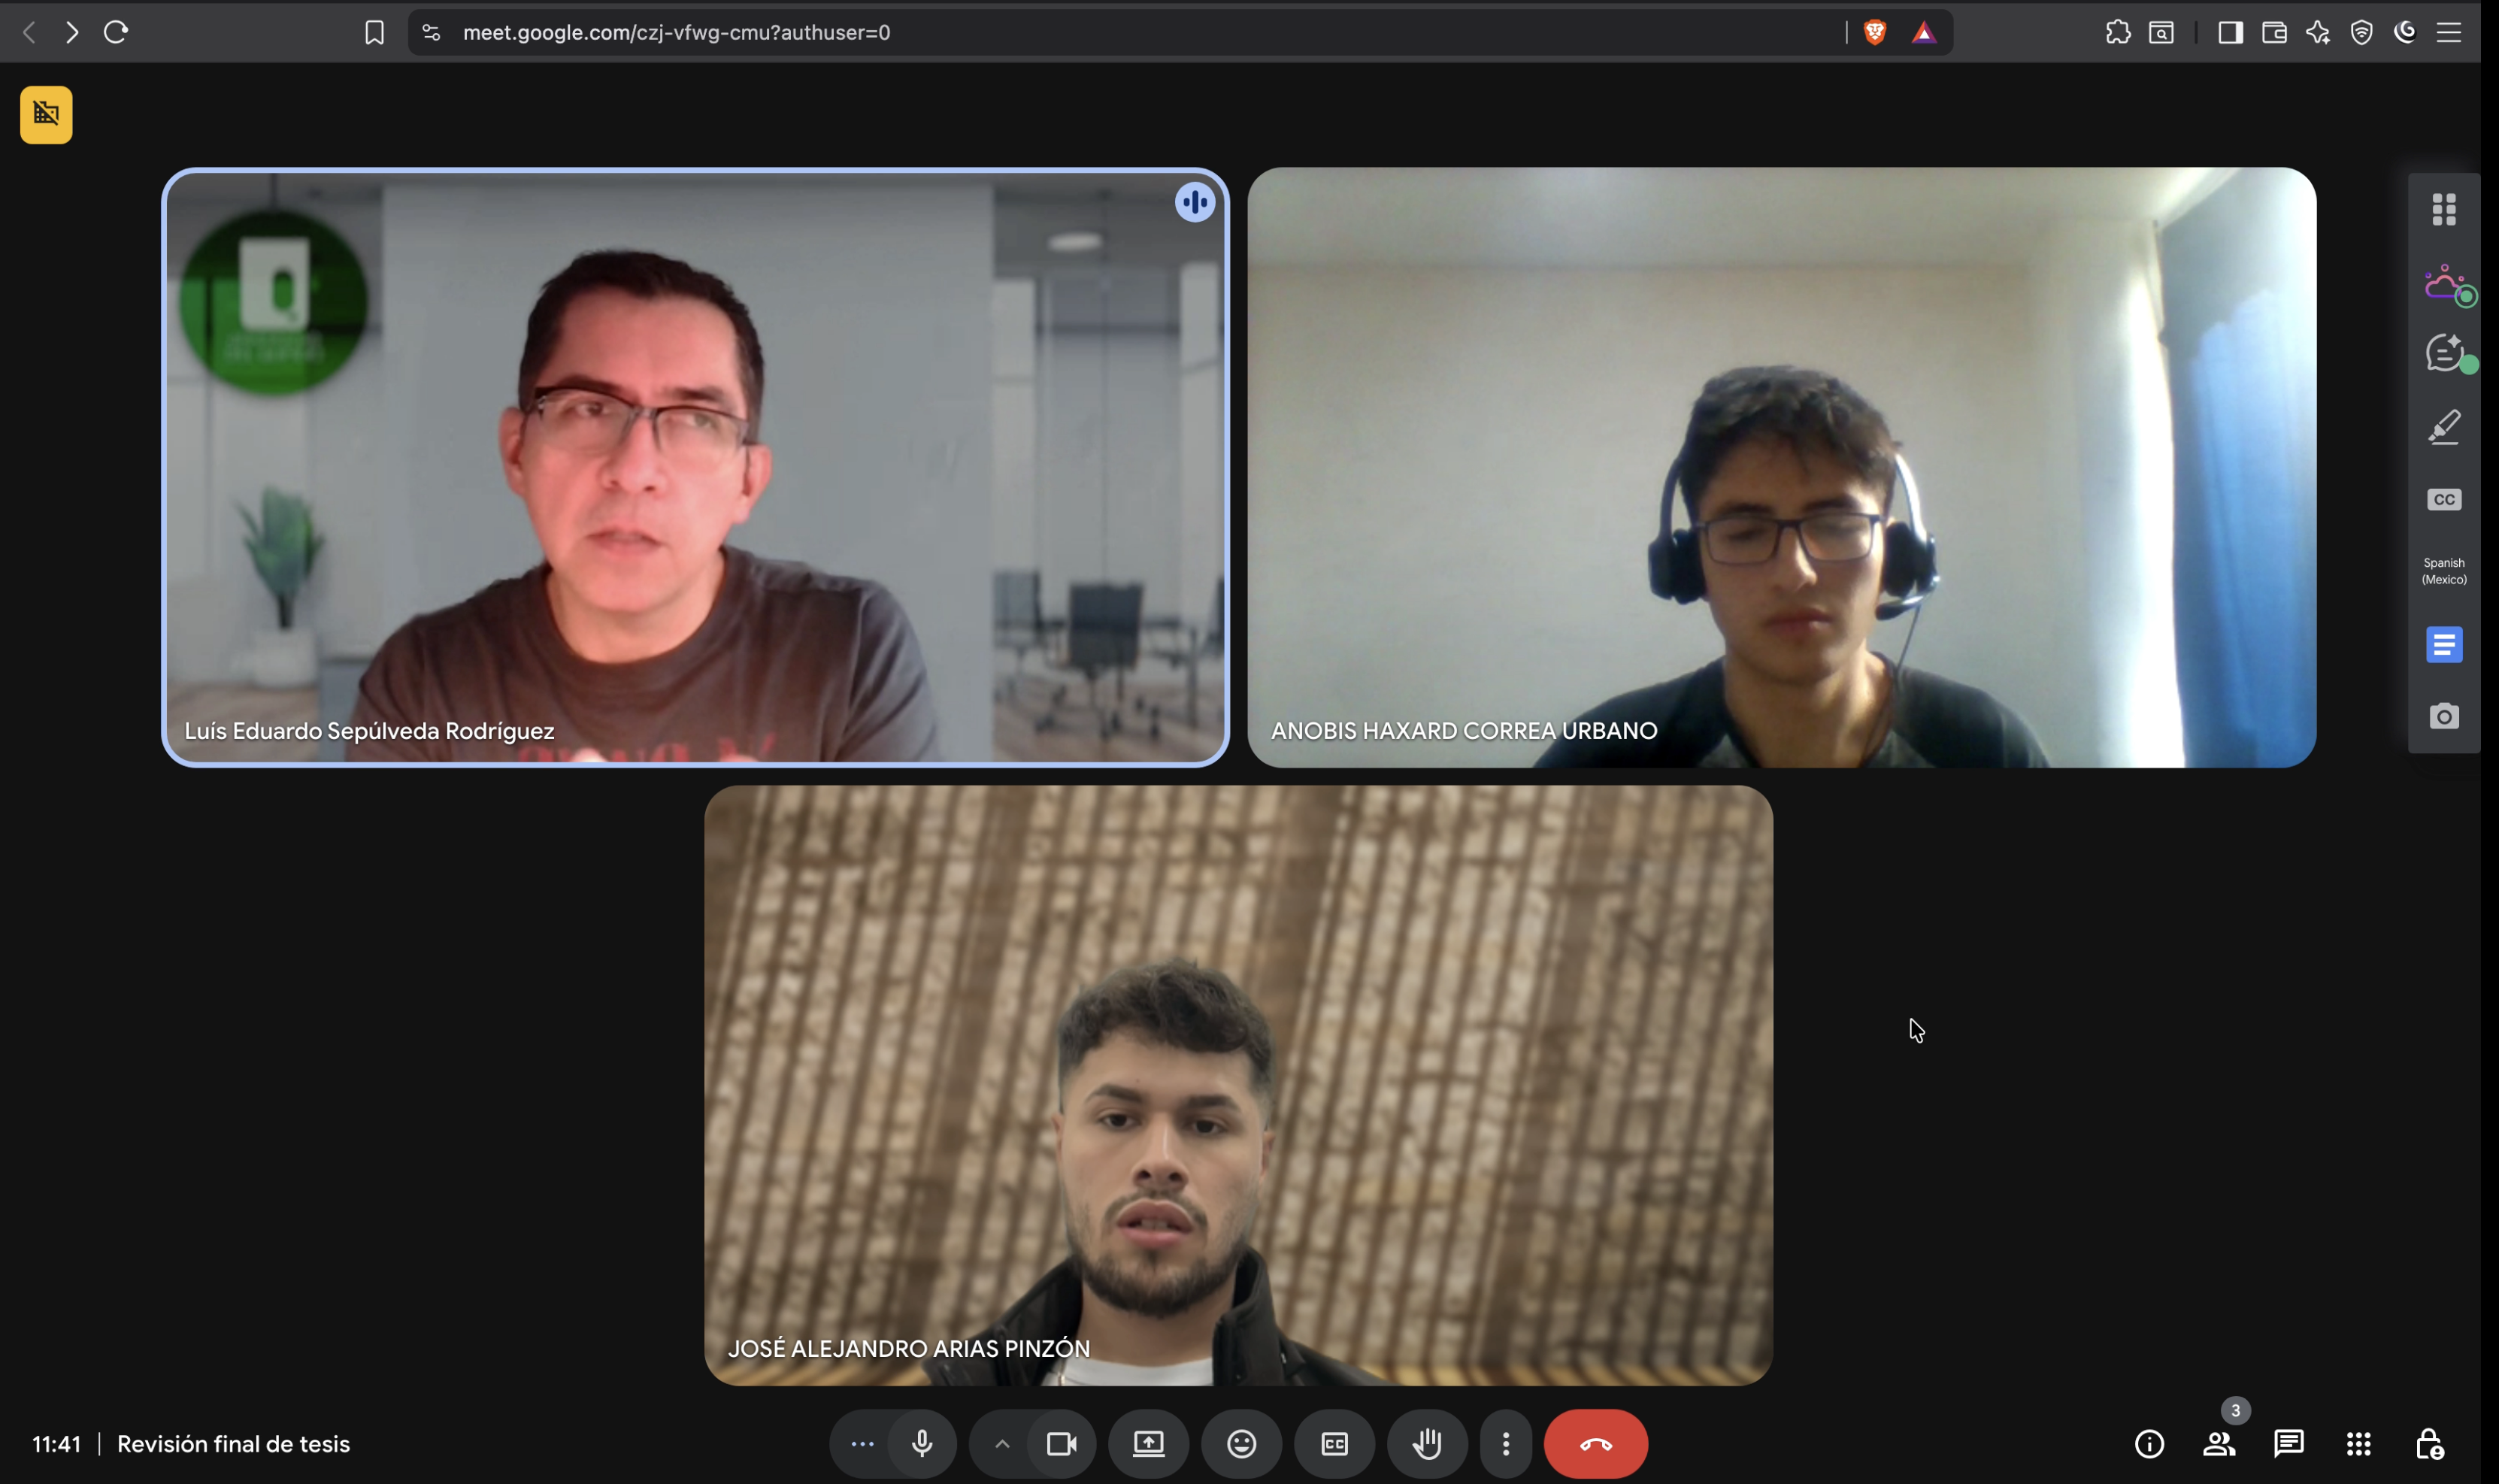
\includegraphics[scale=0.2]{tablas-images/cp6/aceptacion-solucion.png}
    \caption{Captura de pantalla de la reunión de aceptación de la solución}\label{fig:aceptacion-solucion}
\end{figure}
\noindent
Además en el siguiente enlace se puede encontrar la grabación completa de la reunión de aceptación: \href{https://drive.google.com/file/d/1vEsmobYR2ZNxxkTWbN93kyu06ydDNxWd/view?usp=sharing}{aquí}.
\section{Conclusiones de la validación}
\noindent
La validación del \PMV\ permitió corroborar de manera práctica 
y reproducible la solución arquitectónica implementada. Las pruebas 
funcionales automatizadas ---abarcando la creación de clústeres (\texttt{cluster-bootup}), 
la asignación de direcciones IP (\texttt{get-ip}), la gestión de despliegues (\texttt{upload-yaml}) 
y la estrategia de respaldos (\texttt{functional-test/backup})--- demostraron que el sistema 
es capaz de operar en un entorno controlado. Específicamente, 
se validó la correcta integración de los componentes clave (Containerd y K3S) con la 
infraestructura existente del GRID, verificando la persistencia de datos, la orquestación 
de contenedores y la automatización de tareas críticas mediante scripts en Bash y manifiestos YAML. 
La ejecución exitosa de estos casos de prueba, junto con la aceptación formal del docente 
representante, confirma que el \PMV\ no solo satisface los requisitos técnicos y funcionales 
identificados, sino que también se alinea con las necesidades académicas e investigativas 
del GRID, consolidando así la viabilidad de la propuesta como una base sólida para la 
expansión de servicios de virtualización en la Universidad del Quindío.
